\documentclass{beamer}
\setbeamertemplate{caption}[numbered]
\usepackage{phdstyle}

%% image directories
\newcommand{\home}{\string~}
\newcommand{\Artem}{\home/REPOS/COSYINF/img/Artem}
\newcommand{\multisext}{\Artem/multisext_test}
\newcommand{\compare}{\Artem/spin_vs_polarization_fit_comp}
\newcommand{\decoh}{\Artem/decoherence_frequency_dependence}

\title{Spin decoherence in a Frozen Spin lattice, its suppression and effect on the Frequency Domain EDM statistic}
\author{Alexander Aksentev}
\date{\today}

\begin{document}
\begin{frame}
  \titlepage
\end{frame}

\begin{frame}\frametitle{Basic info: T-BMT equation}
  A spin vector placed into a magnetic field is subject to precession described by the T-BMT equation (rest frame):
  \begin{subequations}
    \begin{align}
      \ddt{\vec s} &= \vec s\times \bkt{\vec\W_{MDM} +\vec\W_{EDM}}, \label{eq:TBMT_main}
      \intertext{where MDM and EDM angular velocities $\vec\W_{MDM}$ and $\vec\W_{EDM}$ }
      \vec\W_{MDM} &= \frac qm \bkt*{G\vec B - \bkt{G - \frac{1}{\gamma^2-1}}\frac{\vec E\times\vec\beta}{c}},\label{eq:TBMT_MDM} \\
      \vec\W_{EDM} &= \frac qm \frac\eta2 \bkt*{\frac{\vec E}c + \vec\beta\times \vec B}.\label{eq:TBMT_EDM}
    \end{align}
  \end{subequations}
\end{frame}

\begin{frame}\frametitle{Basic info: Frozen Spin condition}
  From eq.~\eqref{eq:TBMT_MDM} one can observe that the direction of the spin vector can be fixed relative to the momentum vector, i.e., $\vec\W_{MDM}=\vec 0$. This is called the Frozen Spin condition.

  Why is is important?
  \begin{itemize}
  \item In a storage ring, of necessity, $\vec\W_{MDM}\perp \vec\W_{EDM}$
  \item Hence, the measured net angular velocity $\w \propto \sqrt{\W_{MDM}^2 + \W_{EDM}^2} \approx \W_{MDM} + \frac{\W_{EDM}^2}{2\W_{MDM}}$ (EDM is a second-order effect)
  \item When the FS condition is fulfilled, the only remaining (if any) $\vec\W_{MDM}\parallel\vec\W_{EDM}$
  \item Meaning that the EDM-related spin precession frequency shift becomes a first-order effect
  \end{itemize}
\end{frame}

\begin{frame}\frametitle{Basic info: Spin tune and Invariant spin axis}
  The standard formalism operates with spin tune $\nu_s$ and invariant spin axis $\bar n$, defined by the one-turn spin transfer matrix
  \begin{equation*}
    \boldsymbol t_R = \exp\bkt{-i\pi\nu_s\vec\sigma\cdot\bar n} = \cos\pi\nu_s - i(\vec\sigma\cdot\bar n)\sin\pi\nu_s.
  \end{equation*}

  They relate to the spin precession angular velocity as in
  \[
  \vec\W_s = 2\pi f_s\bar n = 2\pi f_R\nu_s\bar n.
  \]

  The invariant spin axis (a.k.a. the spin precession axis) is called such because this is the only direction in which the polarization of a beam survives.
\end{frame}

\begin{frame}\frametitle{Phase stability principle}
  \begin{columns}
    \begin{column}{.5\textwidth}
      \begin{itemize}
      \item In a lattice utilizing an RF cavity, particles travel in bunches
      \item Therefore, the Phase Stability Principle demands that a particle with a longer orbit should have a higher equilibrium-level energy, so that it doesn't fall from the bunch
      \end{itemize}
    \end{column}
    \begin{column}{.5\textwidth}
      \centering
      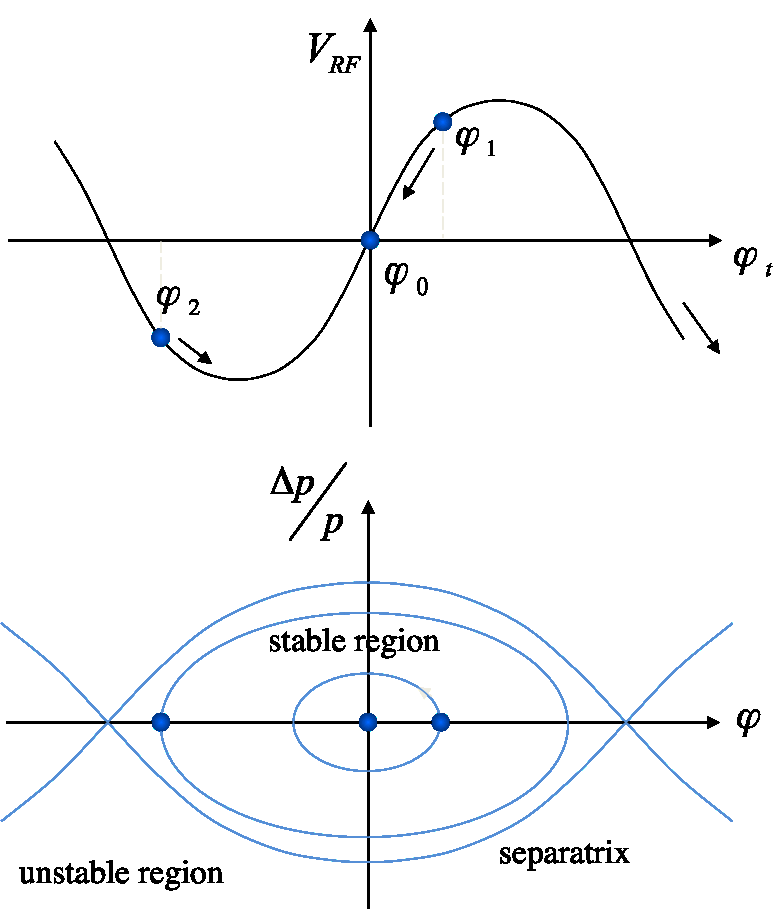
\includegraphics[width=\linewidth]{psp_diagram}
    \end{column}
  \end{columns}
\end{frame}

\begin{frame}\frametitle{Spin tune decoherence}
  \begin{itemize}
  \item Spin tune is proportional to the particle's Lorentz factor: $\nu_s = \gamma G$
  \item Orbit lengthening occurs as a result of:
    \begin{itemize}
    \item Betatron motion: $\bkt{\frac{\Delta L}{L}}_\beta = \frac{\pi}{2L}\bkt*{\varepsilon_xQ_x + \varepsilon_yQ_y}$
    \item Initial momentum deviation: $\bkt{\frac{\Delta L}{L}}_\alpha = \alpha_0\delta + \alpha_1\delta^2 + \dots$
    \end{itemize}
  \item Equilibrium-level momentum shift $\Delta\delta_{eq}$
  \item The particle's Lorentz factor after accounting for the orbit lengthening effects $\gamma_{eff} = \gamma_0 + \beta_0^2\gamma_0\cdor \Delta\delta_{eq}$
  \end{itemize}
\end{frame}

\begin{frame}\frametitle{Sextupole decoherence suppression theory}
  A sextupole of strength
  \[
  S_{sext} = \frac{1}{B\rho} \pddx{B_y}[x][2],
  \]
  has a two-fold effect on decoherence:
  \begin{itemize}
  \item Momentum compaction factor effect: $\Delta \alpha_{1,sext} &= -\frac{S_{sext}D_0^3}{L}$
  \item Orbit length effect: $\bkt{\frac{\Delta L}{L}}_{sext} &= \mp \frac{S_{sext}D_0\beta_{x,y}\varepsilon_{x,y}}{L}$
  \end{itemize}
  Where
  \[
  D(s,\delta) = D_0(s) + D_1(s)\delta
  \]
  is the dispersion function
\end{frame}

\begin{frame}\frametitle{Simulation setup: the beam}
  \begin{itemize}
  \item Flat, normally-distributed beam of 30 particles: $y\sim N(y_0, 0.1)$ mm
  \item $y_0 \in [-1, +1]$ mm
  \item initial spin vector $\vec S(t=0) = (0,0,1)$
  \item Kinetic energy 270.0092 MeV (strict FS)
  \end{itemize}
\end{frame}

\begin{frame}\frametitle{The lattice}
  \begin{columns}
    \begin{column}{.5\textwidth}
      \begin{itemize}
      \item Imperfect Frozen Spin lattice
      \item E+B element tilted about the optic axis by $\theta\sim N(0, 5\cdot 10^{-4})$ rad
      \item Y-family sextupole gradient GSY varied in range $[\mathrm{GSY0} - 5\cdot 10^{-3}, \mathrm{GSY0} + 5\cdot 10^{-3}]$, $\mathrm{GSY0}=-2.5\cdot10^{-3}$ is the optimal setting for the perfect lattice
      \end{itemize}
    \end{column}
    \begin{column}{.5\textwidth}
      \begin{center}
        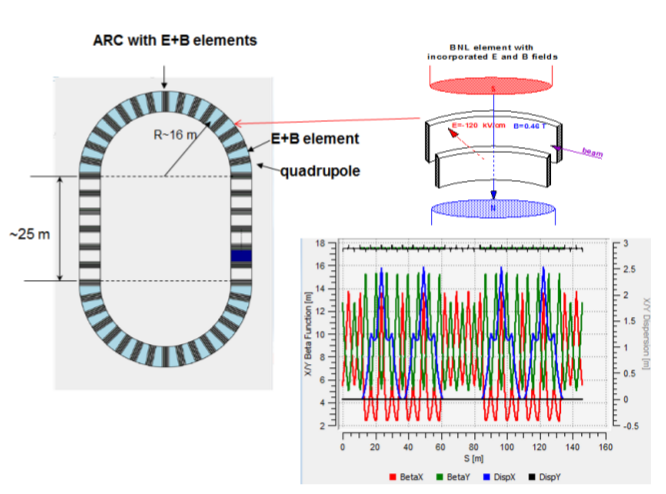
\includegraphics[height=.5\paperheight]{../PhD/img/spin_axis_motion/presentation/lattice}
      \end{center}
    \end{column}
  \end{columns}
\end{frame}

\begin{frame}\frametitle{Tracking parameters and written data}
  \begin{itemize}
  \item Tracking for $1.2\cdot 10^6$ turns (approx. 1.2 sec); data written every 800 turns
  \item Normal Form-computed spin tune and invariant spin axis: $(\nu_s, \bar n_x, \bar n_y, \bar n_z)$
  \item Spin somponents $(S_X, S_Y, S_Z)$
  \item Phase space components $(X, A, Y, B, T, D)$
  \end{itemize}
\end{frame}

\begin{frame}\frametitle{Computed data}
  \begin{itemize}
  \item Polarization $\vec P = \frac{\sum_i\vec S_i}{|\sum_i\vec S_i|}$
  \item Model  $f(t; a,f,\phi) = a\cdot \sin(2\pi\cdot f\cdot t + \phi)$
  \item Fitted parameters:  $(\hat a, \hat f, \hat\phi)$
  \end{itemize}
\end{frame}

\begin{frame}\frametitle{Spin precession axis effect}
  \begin{figure}[H]
    \centering
    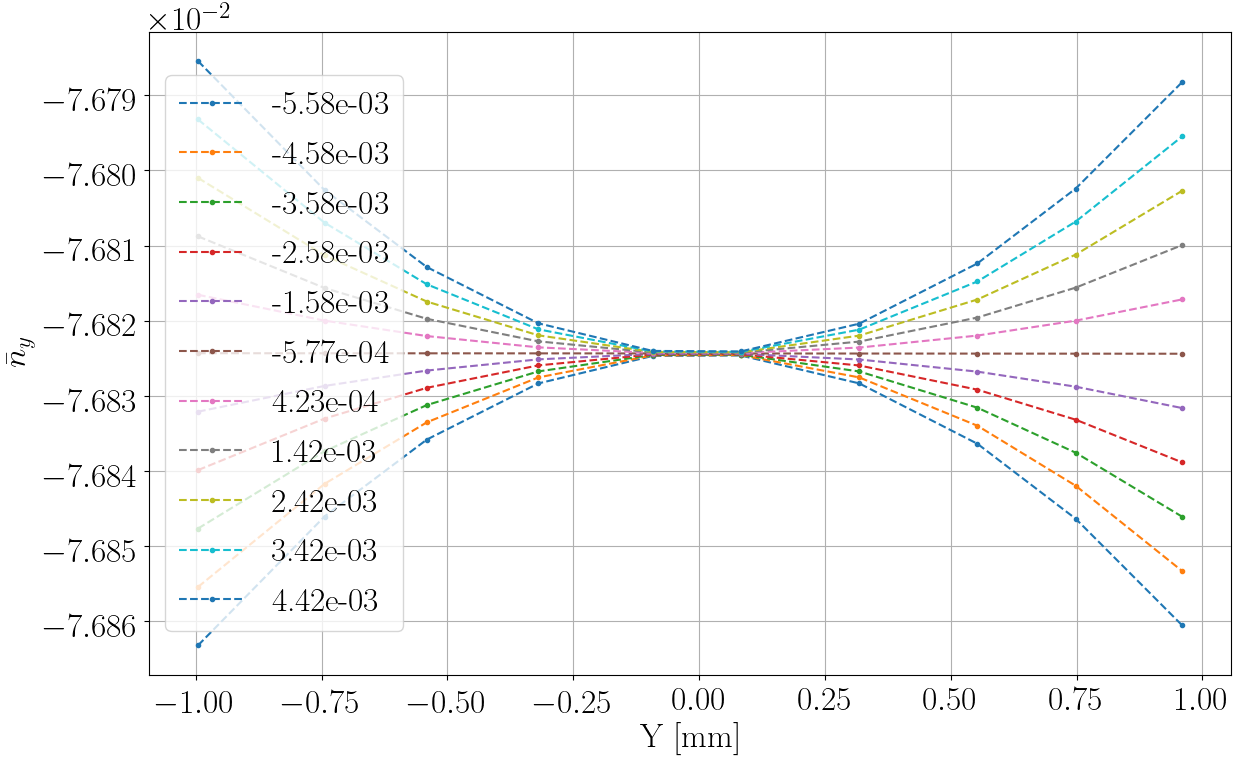
\includegraphics[width=\linewidth]{\multisext/ny_vs_offset}
    \caption{SPA component $\bar n_y$ as a function of the vertical particle offset, sextupole gradient value.\label{fig:DECOH_full_ny}}
  \end{figure}
\end{frame}

\begin{frame}\frametitle{SPA: zoom}
  \begin{figure}[H]
    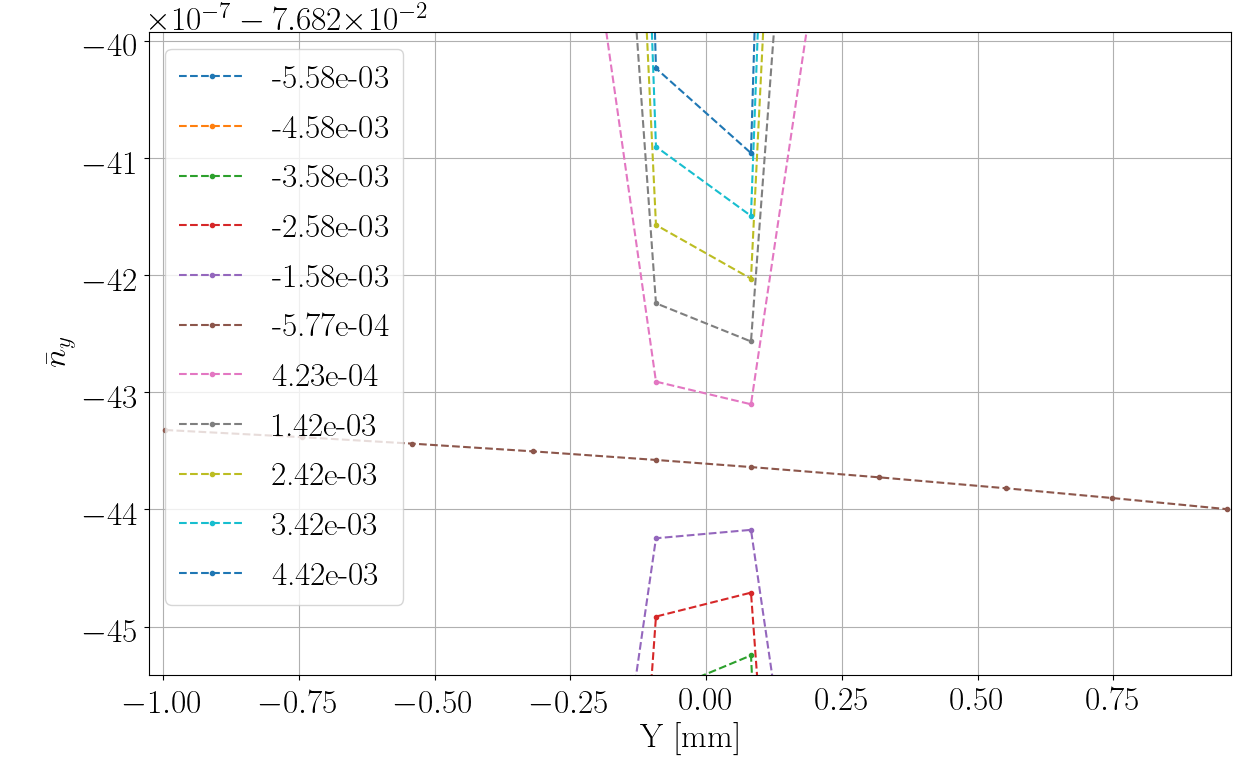
\includegraphics[width=\linewidth]{\multisext/ny_vs_offset_zoom}
    \caption{Zoom of Figure~\ref{fig:DECOH_full_ny}. SPA component $\bar
      n_y$ (as well as $\bar n_x$) is a parabola in the neighborhood of the reference orbit at
      the optimal GSY value, unlike $\nu_s$, which is \textbf{linear}.}
  \end{figure}
\end{frame}

\begin{frame}\frametitle{Spin tune effect}
  \begin{figure}[H]
    \centering
    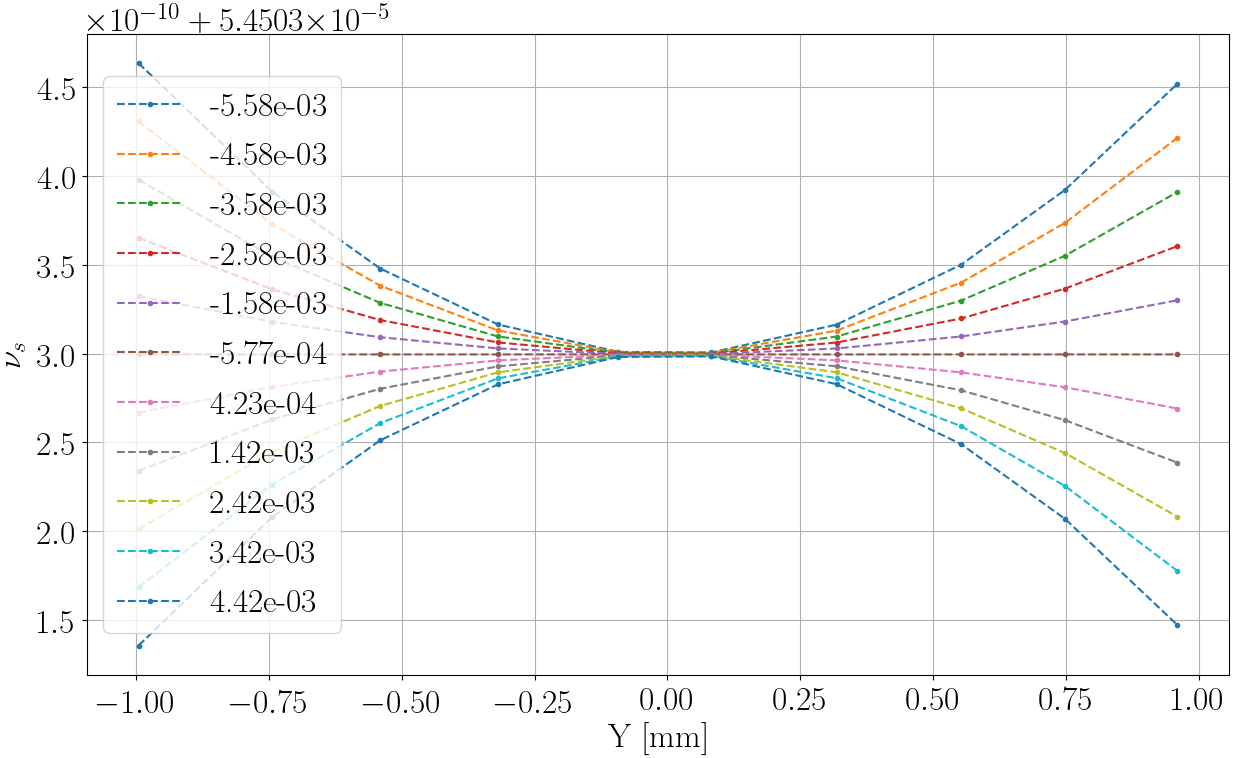
\includegraphics[width=\linewidth]{\multisext/spin_tune_vs_offset}
    \caption{Spin tune $\nu_s$ Taylor expansion contains a linear term insensitive to sextupole optimization.\label{fig:SpinTune_vs_Y0_GSY}}
  \end{figure}
\end{frame}
\begin{frame}\frametitle{Frequency estimate effect}
  Fitted data: Polarization.
  \begin{figure}[H]
    \centering
    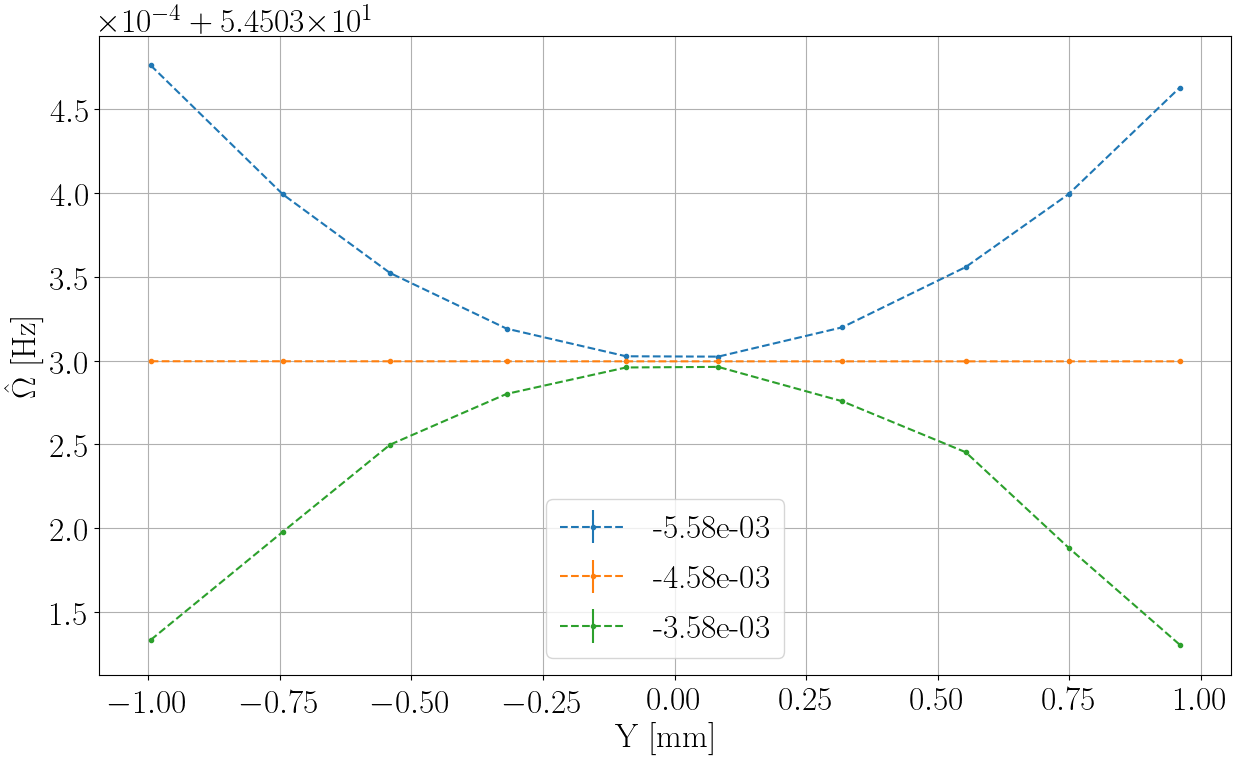
\includegraphics[width=\linewidth]{\multisext/FreqY_vs_offset}
    \caption{Frequency estimate for the optimal sextupole gradient (orange) and the values at the ends of the searched range.\label{fig:FreqY_vs_offset}}
  \end{figure}
\end{frame}
\begin{frame}\frametitle{Frequency estimate: zoom}
  \begin{figure}[H]
    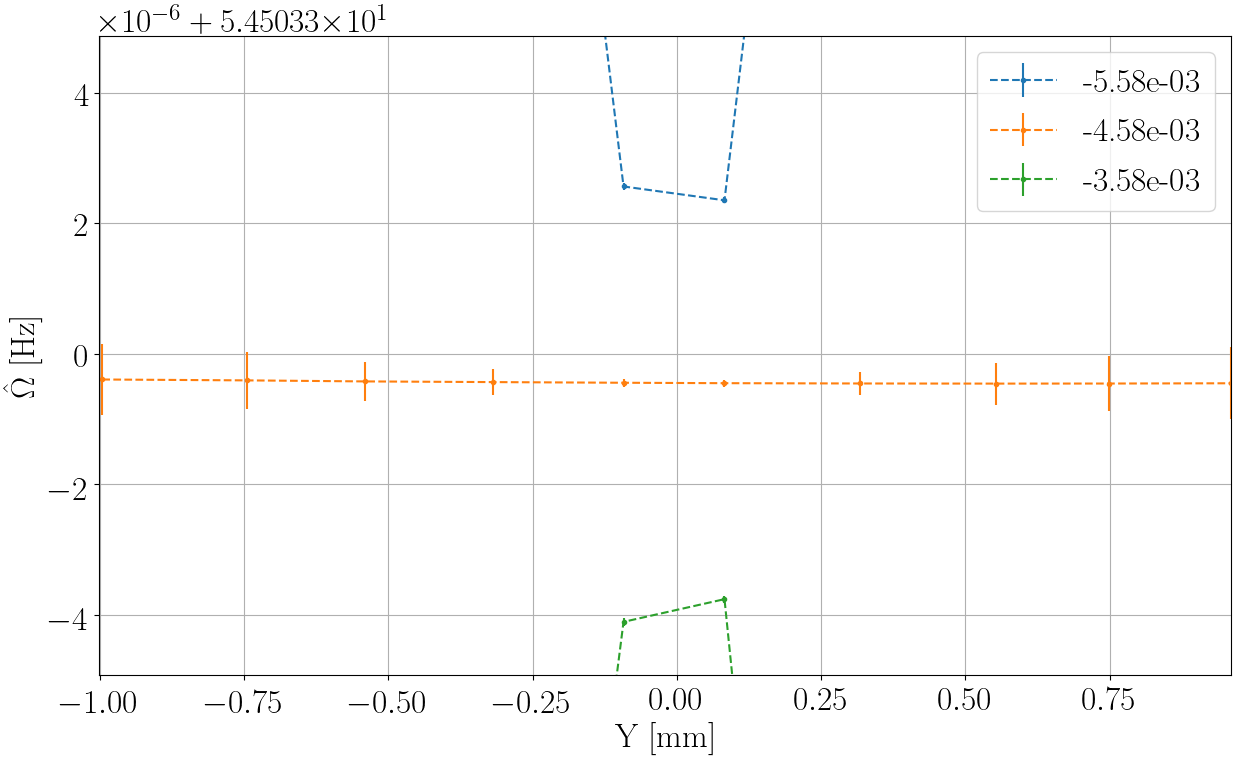
\includegraphics[width=\linewidth]{\multisext/FreqY_vs_offset_zoom}
    \caption{Zoom of Figure~\ref{fig:FreqY_vs_offset}. Frequency estimate depends on the offset value linearly,
      like  $\nu_s$, and unlike $\bar n_y$.}
  \end{figure}
\end{frame}

\begin{frame}\frametitle{Individual particle ST+SPA structure}
  \begin{figure}[H]
  \centering
  \includegraphics[width=\linewidth]{\decoh/ny_vs_turn}
  \caption{SPA component $\bar n_y$ for \textbf{particles} with offsets:
    [1.02749, 1.02937, 1.02840] mm. We observe small-amplitude rapid oscillations about
    an average level. This average level changes parabolically with the vertical
    offset (Figure~\ref{fig:mean_tune_axis} below). The rapid oscillations are
    due to betatron motion (Figures~\ref{fig:tune_axis_position_y},
    and~\ref{fig:tune_axis_position_x}).\label{fig:ny_vs_turn}}
\end{figure}
\end{frame}

\begin{frame}\frametitle{Vertical betatron motion dependence}
  \begin{figure}[H]
    \centering
    \begin{subfigure}[t]{.5\textwidth}
      \includegraphics[width=\linewidth]{\decoh/ny_vs_y}
      \caption{SPA component $\bar n_y$ as a function of the vertical particle position.}
    \end{subfigure}~
    \begin{subfigure}[t]{.5\textwidth}
      \includegraphics[width=\linewidth]{\decoh/spin_tune_vs_y}
      \caption{Spin tune $\nu_s$ as a function of the vertical particle position.}
    \end{subfigure}
    \caption{Particle spin precession frequency depending on its vertical position.
      The observed non-functionality of the parameters on the $y$-position os due to the dependence on the $x$-position as well, which also oscillates at a small amplitude (Figure~\ref{fig:tune_axis_position_x}). \label{fig:tune_axis_position_y}}
  \end{figure}
\end{frame}

\begin{frame}\frametitle{Horizontal betatron motion dependence}
  \begin{figure}[H]
    \centering
    \begin{subfigure}[t]{.5\textwidth}
      \includegraphics[width=\linewidth]{\decoh/ny_vs_x}
      \caption{SPA component $\bar n_y$ as a function of the horizontal particle position.}
    \end{subfigure}~
    \begin{subfigure}[t]{.5\textwidth}
      \includegraphics[width=\linewidth]{\decoh/spin_tune_vs_x}
      \caption{Spin tune $\nu_s$ as a function of the horizontal particle position.}
    \end{subfigure}
    \caption{Particle spin precession frequency as a function of its radial position.\label{fig:tune_axis_position_x}}
  \end{figure}
\end{frame}

\begin{frame}
  \begin{figure}[H]
    \centering
    \includegraphics[width=\linewidth]{\decoh/mean_spin_tune_vs_offset}
    \caption{Mean level of spin tune as a function of beam offset}
  \end{figure}
\end{frame}

\begin{frame}
  \begin{figure}[H]
    \includegraphics[width=\linewidth]{\decoh/mean_nbar_vs_mean_spin_tune}
    \caption{Mean SPA and ST levels versus each other. Observe a strong correlation.\label{fig:mean_tune_axis}}
  \end{figure}
\end{frame}

\begin{frame}\frametitle{Frequency estimate offset dependence}
  Fitted data: spin.
  \begin{figure}[H]
    \centering
    \includegraphics[width=\linewidth]{\decoh/freqY_vs_offset}
    \caption{$\hat f$ as a function of the initial vertical offset.}
  \end{figure}
\end{frame}

\begin{frame}\frametitle{Spin tune dependence}
  \begin{figure}[H]
    \includegraphics[width=\linewidth]{\decoh/freqY_vs_mean_spin_tune}
    \caption{$\hat f$ as a function of the mean spin tune level.}
  \end{figure}
\end{frame}

\begin{frame}
  \begin{figure}[H]
    \includegraphics[width=\linewidth]{\decoh/freqY_vs_abs_offset}
    \caption{$\hat f$ as a function of the absolute value of the initial vertical offset.}
  \end{figure}
\end{frame}

\begin{frame}
  \begin{center}
    Thank you!
  \end{center}
\end{frame}
\end{document}
